\documentclass[a4paper, 12pt]{article}

%%% Работа с русским языком
\usepackage{cmap}					% поиск в PDF
\usepackage{mathtext} 				% русские буквы в формулах
\usepackage[T2A]{fontenc}			% кодировка
\usepackage[utf8]{inputenc}			% кодировка исходного текста
\usepackage[russian]{babel}	% локализация и переносы

%%% Дополнительная работа с математикой
\usepackage{amsmath,amsfonts,amssymb,amsthm,mathtools} % AMS
\usepackage{icomma} % "Умная" запятая: $0,2$ --- число, $0, 2$ --- перечисление

%% Номера формул
%\mathtoolsset{showonlyrefs=true} % Показывать номера только у тех формул, на которые есть \eqref{} в тексте.

%% Шрифты
\usepackage{euscript}	 % Шрифт Евклид
\usepackage{mathrsfs} % Красивый матшрифт

%% Поля
\usepackage[left=2cm,right=2cm,top=2cm,bottom=2cm,bindingoffset=0cm]{geometry}

%% Русские списки
\usepackage{enumitem}
\makeatletter
\AddEnumerateCounter{\asbuk}{\russian@alph}{щ}
\makeatother

%%% Работа с картинками
\usepackage{graphicx}  % Для вставки рисунков
\graphicspath{{images/}{images2/}}  % папки с картинками
\setlength\fboxsep{3pt} % Отступ рамки \fbox{} от рисунка
\setlength\fboxrule{1pt} % Толщина линий рамки \fbox{}
\usepackage{wrapfig} % Обтекание рисунков и таблиц текстом

%%% Работа с таблицами
\usepackage{array,tabularx,tabulary,booktabs} % Дополнительная работа с таблицами
\usepackage{longtable}  % Длинные таблицы
\usepackage{multirow} % Слияние строк в таблице

%% Красная строка
\setlength{\parindent}{2em}

%% Интервалы
\linespread{1}
\usepackage{multirow}

%% TikZ
\usepackage{tikz}
\usetikzlibrary{graphs,graphs.standard}

%% Верхний колонтитул
\usepackage{fancyhdr}
\pagestyle{fancy}

%% Перенос знаков в формулах (по Львовскому)
\newcommand*{\hm}[1]{#1\nobreak\discretionary{}
	{\hbox{$\mathsurround=0pt #1$}}{}}

%% Мои дополнения
\usepackage{float} %Добавляет возможность работы с командой [H] которая улучшает расположение на странице
\usepackage{gensymb} %Красивые градусы
\usepackage{graphicx}               % Импорт изображений
\usepackage{caption} % Пакет для подписей к рисункам, в частности, для работы caption*


\begin{document}

\newcommand{\HRule}{\rule{\linewidth}{0.7mm}} % Defines a new command for the horizontal lines, change thickness here
	
	\begin{center}
		\large\textbf{Московский Физико-Технический Институт}\\
		\large\textbf{(государственный университет)}
	
		\vfill
		
		\Large Лабораторная работа по курсу общей физики № 3.2.8\\[0.5cm] % Minor heading such as course title
		
		%----------------------------------------------------------------------------------------
		%	TITLE SECTION
		%----------------------------------------------------------------------------------------
		
		\HRule
		\\[0.4cm]
		{ \huge \bfseries Релаксационные колебания}
		\\[0.4cm] % Title of your document
		\HRule
		\\[0.5cm]
		
		\ \\
	\textbf{\large Автор:} \\	
	\large Баранников Андрей Б01-001\\
		\vfill
		\hspace*{-0.8 cm}
\includegraphics[width=100 pt]{frkt_logo}\\
		\large Долгопрудный, 2021
	\end{center}

\newpage
\setcounter{page}{2}
\fancyfoot[c]{\thepage}
\fancyhead[L] {Работа 3.2.8}
\fancyhead[R]{}

\newpage

\noindent \textbf{Цель работы:} 
\noindent изучение вольт-амперной характеристики нормального тлеющего разряда; исследование релаксационного генератора на стабилитроне.\\
\noindent \textbf{В работе используются:} 
\noindent стабилитрон СГ-2 (газонаполненный диод) на монтажной панели, амперметр, магазин сопротивлений, магазин ёмкостей, источник питания, осциллограф (ЭО), генератор звуковой частоты (ЗГ).
\section*{Описание работы}



\begin{figure}[h!]
	\centering
	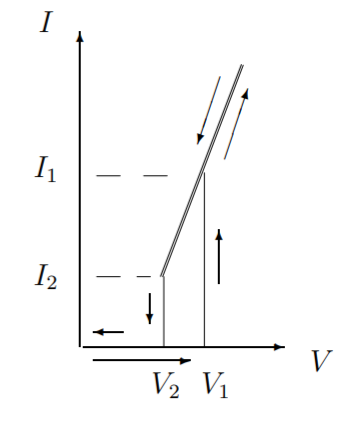
\includegraphics[scale=0.8]{image_1.png}
	\caption{Вольтамперная характеристика стабилитрона с последовательно включенным резистором\label{fig:image_1}}
	
\end{figure}

Зависимость тока от напряжения для газоразрядной лампы не подчиняется закону Ома и характеризуется рядом особенностей, ее вольтамперная характеристика указана на \textit{рис. \ref{fig:image_1}}

При малых напряжениях лампа практически не пропускает ток. Как только разность потенциалов на ее электродах достигает напряжения зажигания в лампе начинает течь ток. После, так как наш источник напряжения не может поддерживать такую силу тока, напряжение на лампе начинает падать и достигая напряжения гашения, силу тока на ней скачком падает до нуля.

\begin{figure}[h!]
	\centering
	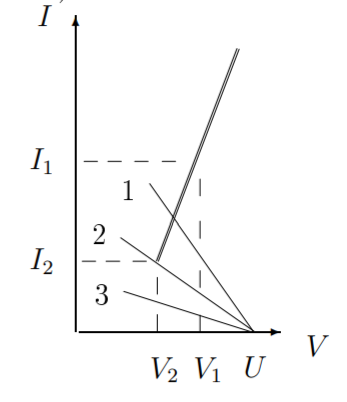
\includegraphics[scale=0.8]{image_3.png}
	\caption{Режимы работы релаксационного генератора}
	\label{fig:image_2}
\end{figure}

Колебательный процесс возможен когда нагрузочная прямая не пересекает характеристику лампы (3 прямая на \textit{рис. \ref{fig:image_2}}). Это происходит из-за того, что в стационарном режиме ток через лампу равен:

\[I_{ст} = \frac{U - V}{R},\]

где $V$ - напряжение на конденсаторе и оно постоянно. Тогда прямая 2 проходящая через точку $(I_2, V_2)$, соответствует критическому сопротивлению:

\[R_{кр} = \frac{U - V_2}{I_2},\]

тогда для $R > R_{кр}$ в системе установятся колебания.

\begin{figure}[h!]
	\centering
	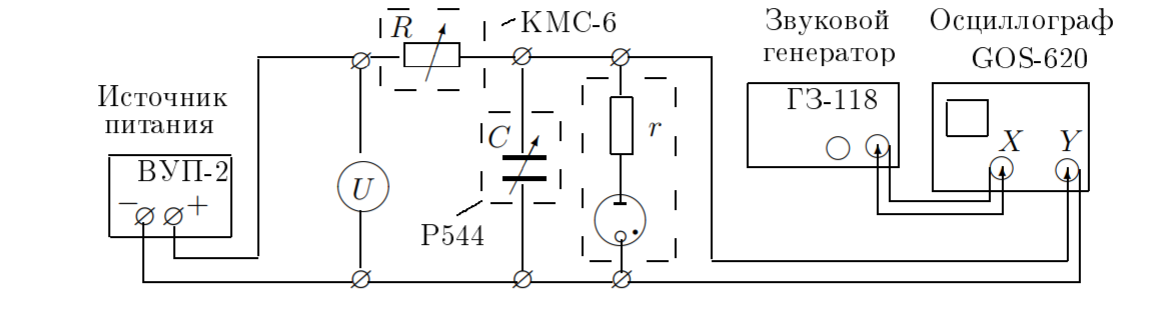
\includegraphics[scale=0.8]{image_2.png}
	\caption{Схема установки для изучения релаксационных колебаний}
	\label{fig:image_3}
\end{figure}

Схема установки изображена на \textit{рис. \ref{fig:image_3}}. Здесь период колебаний будет складываться из времени заряда $\tau_{\textit{з}}$ и времения разряда $\tau_{\textit{р}}$. В случае, когда сопротивление $R$ существенно превосходит внутреннее сопротивление стабилитрона, справедливо соотношение $\tau_{\textit{з}} \gg \tau_{\textit{р}}$. В таком случае период колебаний можно посчитать при помощи такой формулы:

\begin{equation}
	T \approx \tau_{з} = RC\ln \frac{U - V_2}{U - V_1},
\end{equation}

где $V_1$ и $V_2$ потенциалы зажигания и гашения соответственно.

\newpage

\section*{Ход работы}\

Снимем вольтамперную характеристику стабилитрона, внутреннее сопротивление стабилитрона $r = 5,1 \, кОм$. Запишем данные в таблицу для систем из стабилитрона и дополнительного сопротивления $r$ и для стабилитрона без сопротивления $r$. Построим графики зависимости $I = f(V)$ по данным таблицам.


\begin{table}[!h]
	\begin{minipage}[h]{0.5\linewidth}
	\centering
	\begin{tabular}{|cc|cc|c}
		\cline{1-4}
		\multicolumn{2}{|c|}{С   учётом r}                         & \multicolumn{2}{c|}{Без   учёта r}                        &                                                  \\ \cline{1-4}
		\multicolumn{1}{|c|}{U, В}                         & I, мА & \multicolumn{1}{c|}{U, В}                         & I, мА &                                                  \\ \cline{1-4}
		\multicolumn{1}{|c|}{41,7}                         & 0,0   & \multicolumn{1}{c|}{41,7}                         & 0,0   &                                                  \\ \cline{1-4}
		\multicolumn{1}{|c|}{50,8}                         & 0,0   & \multicolumn{1}{c|}{50,8}                         & 0,0   &                                                  \\ \cline{1-4}
		\multicolumn{1}{|c|}{59,8}                         & 0,0   & \multicolumn{1}{c|}{59,8}                         & 0,0   &                                                  \\ \cline{1-4}
		\multicolumn{1}{|c|}{71,8}                         & 0,0   & \multicolumn{1}{c|}{71,8}                         & 0,0   &                                                  \\ \cline{1-4}
		\multicolumn{1}{|c|}{82,3}                         & 0,0   & \multicolumn{1}{c|}{82,3}                         & 0,0   &                                                  \\ \hline
		\rowcolor[HTML]{F8CBAD} 
		\multicolumn{1}{|c|}{\cellcolor[HTML]{F8CBAD}88,2} & 2,2   & \multicolumn{1}{c|}{\cellcolor[HTML]{F8CBAD}77,0} & 2,2   & \multicolumn{1}{c|}{\cellcolor[HTML]{F8CBAD}$V_1$} \\ \hline
		\multicolumn{1}{|c|}{97,3}                         & 3,5   & \multicolumn{1}{c|}{79,7}                         & 3,5   &                                                  \\ \cline{1-4}
		\multicolumn{1}{|c|}{108,5}                        & 5,1   & \multicolumn{1}{c|}{82,5}                         & 5,1   &                                                  \\ \cline{1-4}
		\multicolumn{1}{|c|}{97,2}                         & 3,4   & \multicolumn{1}{c|}{79,8}                         & 3,4   &                                                  \\ \hline
		\rowcolor[HTML]{B4C6E7} 
		\multicolumn{1}{|c|}{\cellcolor[HTML]{B4C6E7}84,2} & 1,6   & \multicolumn{1}{c|}{\cellcolor[HTML]{B4C6E7}76,0} & 1,6   & \multicolumn{1}{c|}{\cellcolor[HTML]{B4C6E7}$V_2$} \\ \hline
	\end{tabular}
	\caption{Зависимость $U(I)$. $V_1$ - напряжение зажигания, $V_2$ - напряжение гашения}
	\label{tab:table_1}
	\end{minipage}
	\begin{minipage}[h]{0.5\linewidth}
		\center{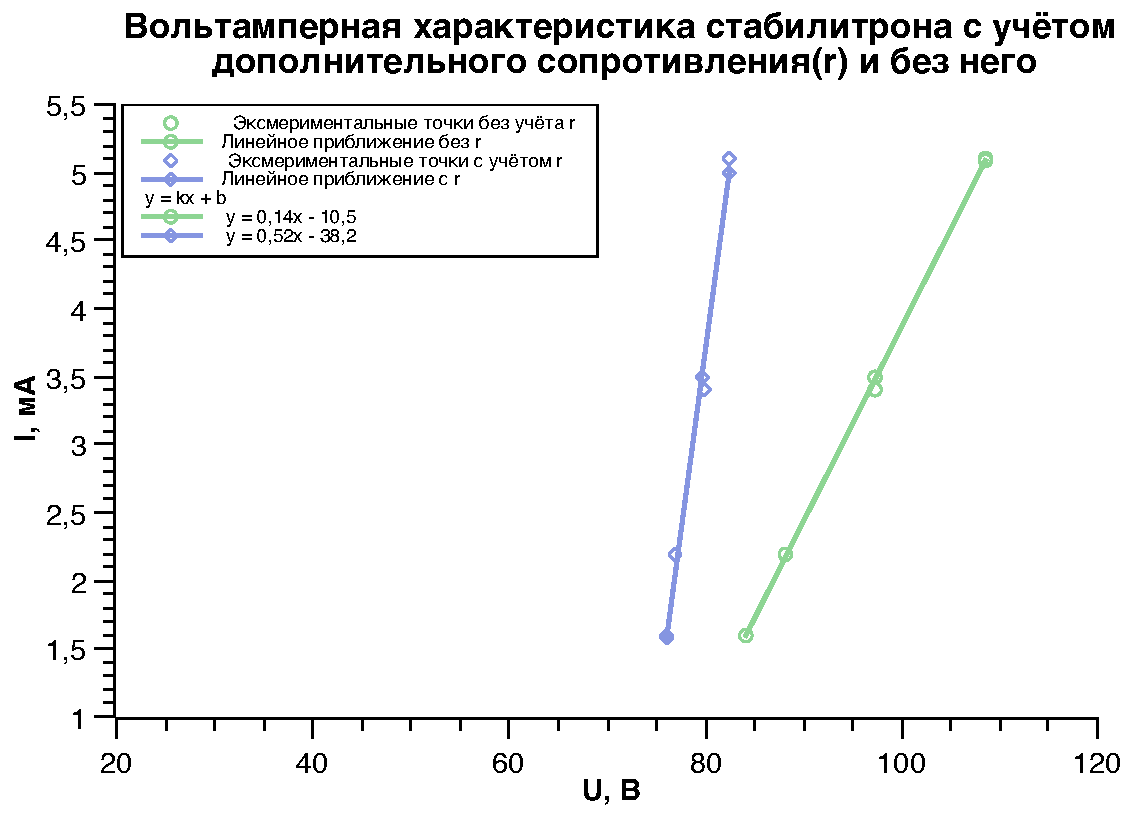
\includegraphics[width=\textwidth]{plot_1} График $I = f(V)$}
	\end{minipage}
\end{table}

Соберем релаксационный генератор. Подберем частоту развертки так, чтобы было видно пилообразную картинку.  Отношение времени зарядки к времени разрядки $\tau_{з}/\tau_{р} = 15$. 

\begin{figure}[h!]
	\centering
	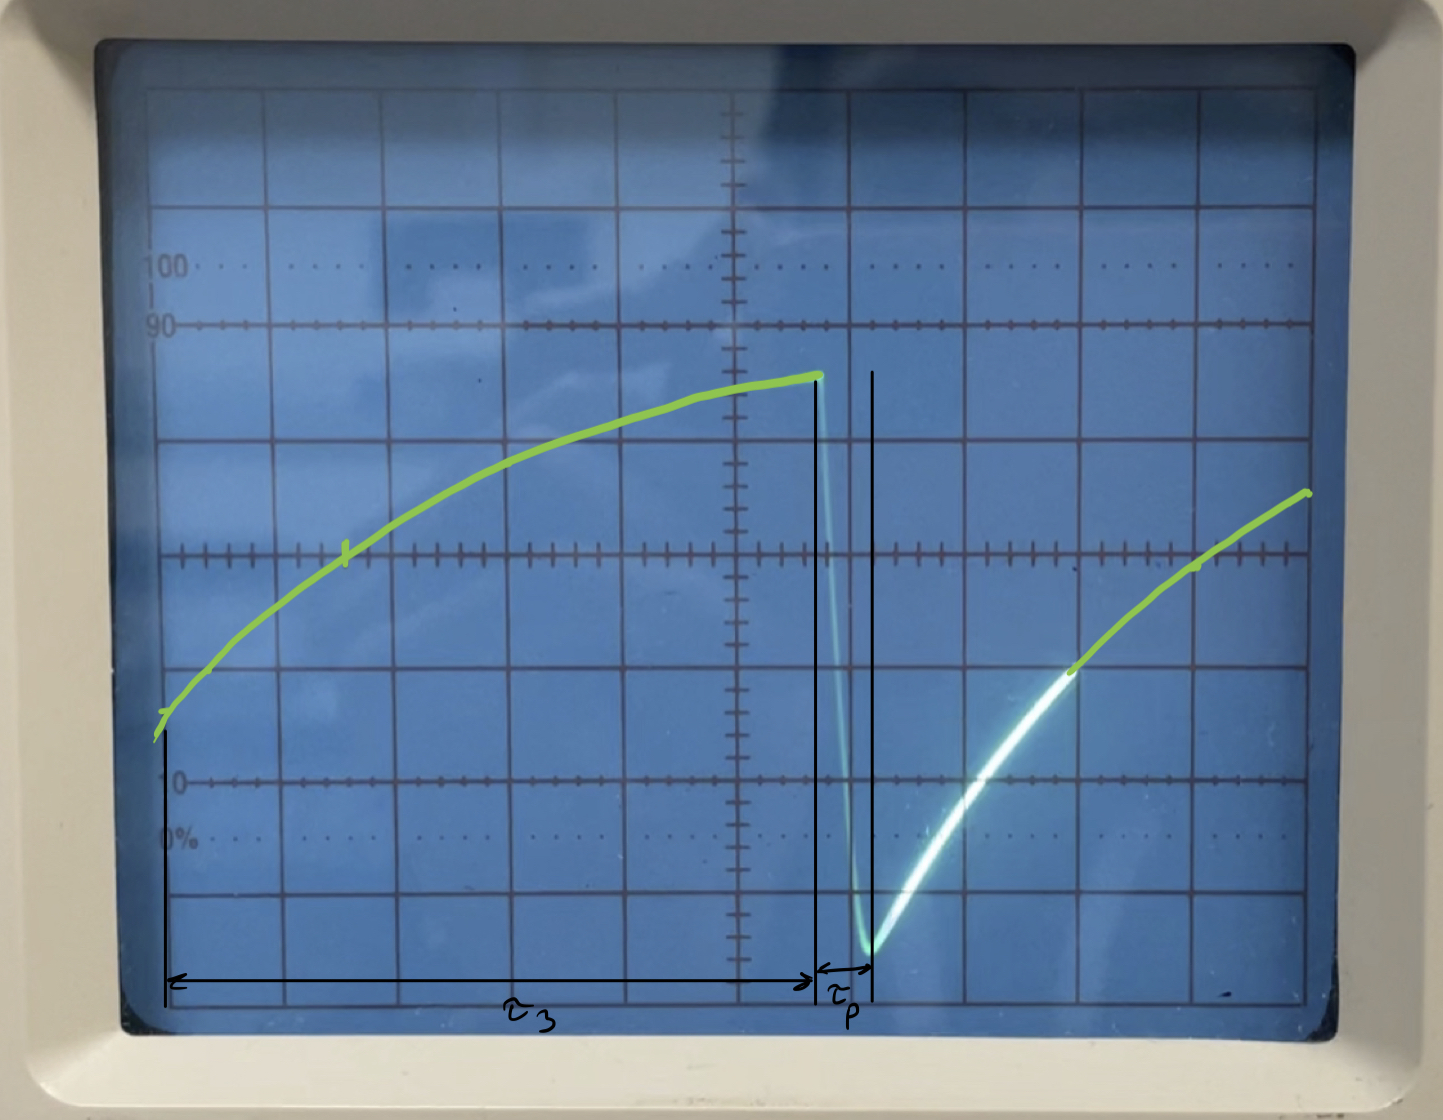
\includegraphics[width=0.6\textwidth]{image_4}
	\caption{Пилообразная картинка}
	\label{fig:image_4}
\end{figure}

Уменьшая сопротивление магазина определим $R_{кр}$, при котором пропадают колебания. $R_{кр} = 115$ кОм, при этом теоретическое значение критического сопротивления $R_\textit{теор} = 23$ кОм. Такие различия возникают в результате неидеальности схемы и возникновения в ней помех.

\newpage

Подадим сигнал с генератора на вход \textit{Х} осциллографа. Меняя частоту ЗГ получим на экране фигуру Лиссажу без самопересечений. Не меняя параметров релаксационного генератора получим фигуры Лиссажу при соотношении частот 2:1, 3:1, 1:2, 1:3.

\begin{figure}[!h]
	\begin{minipage}[h]{0.45\linewidth}
		\center{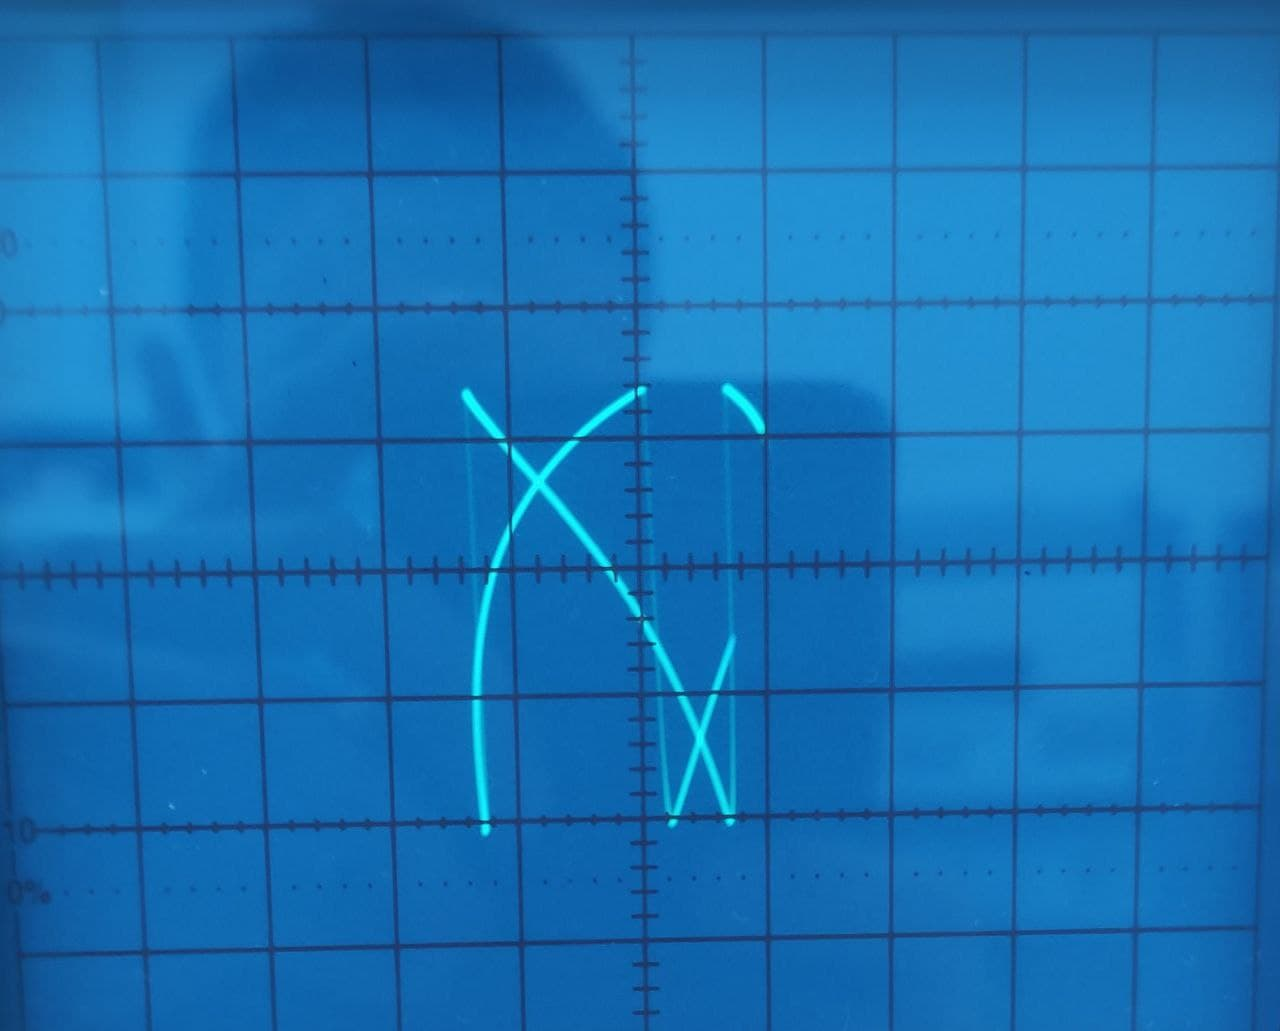
\includegraphics[width=\textwidth]{image_3-1} Соотношение сторон 3:1}
	\end{minipage}
\hfill
	\begin{minipage}[h]{0.45\linewidth}
		\center{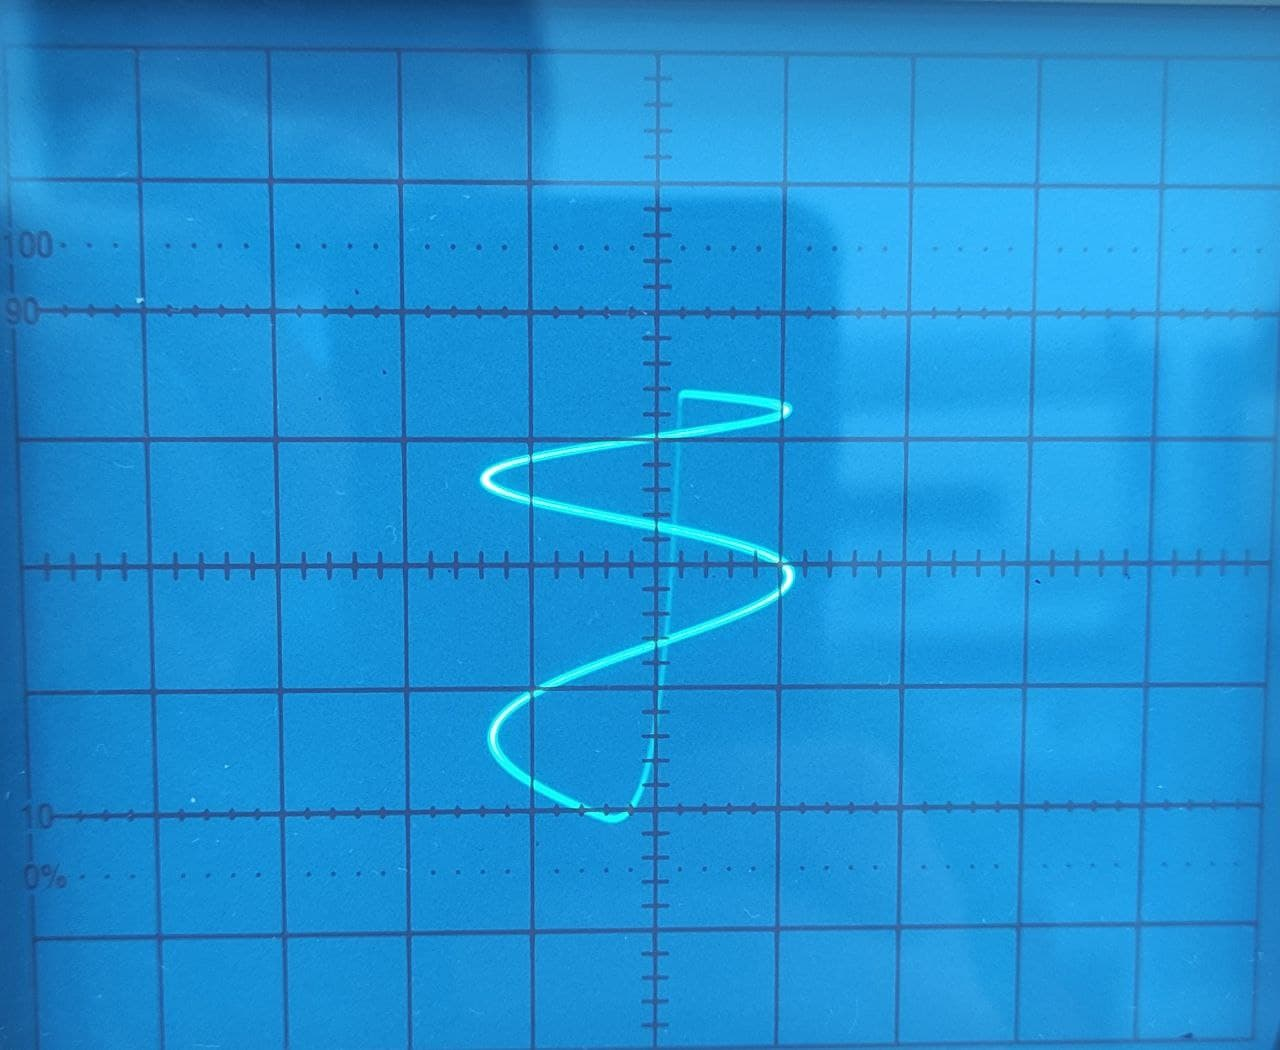
\includegraphics[width=\textwidth]{image_1-2} Соотношение сторон 1:2}
	\end{minipage}
\vfill
	\begin{minipage}[h]{0.45\linewidth}
	\center{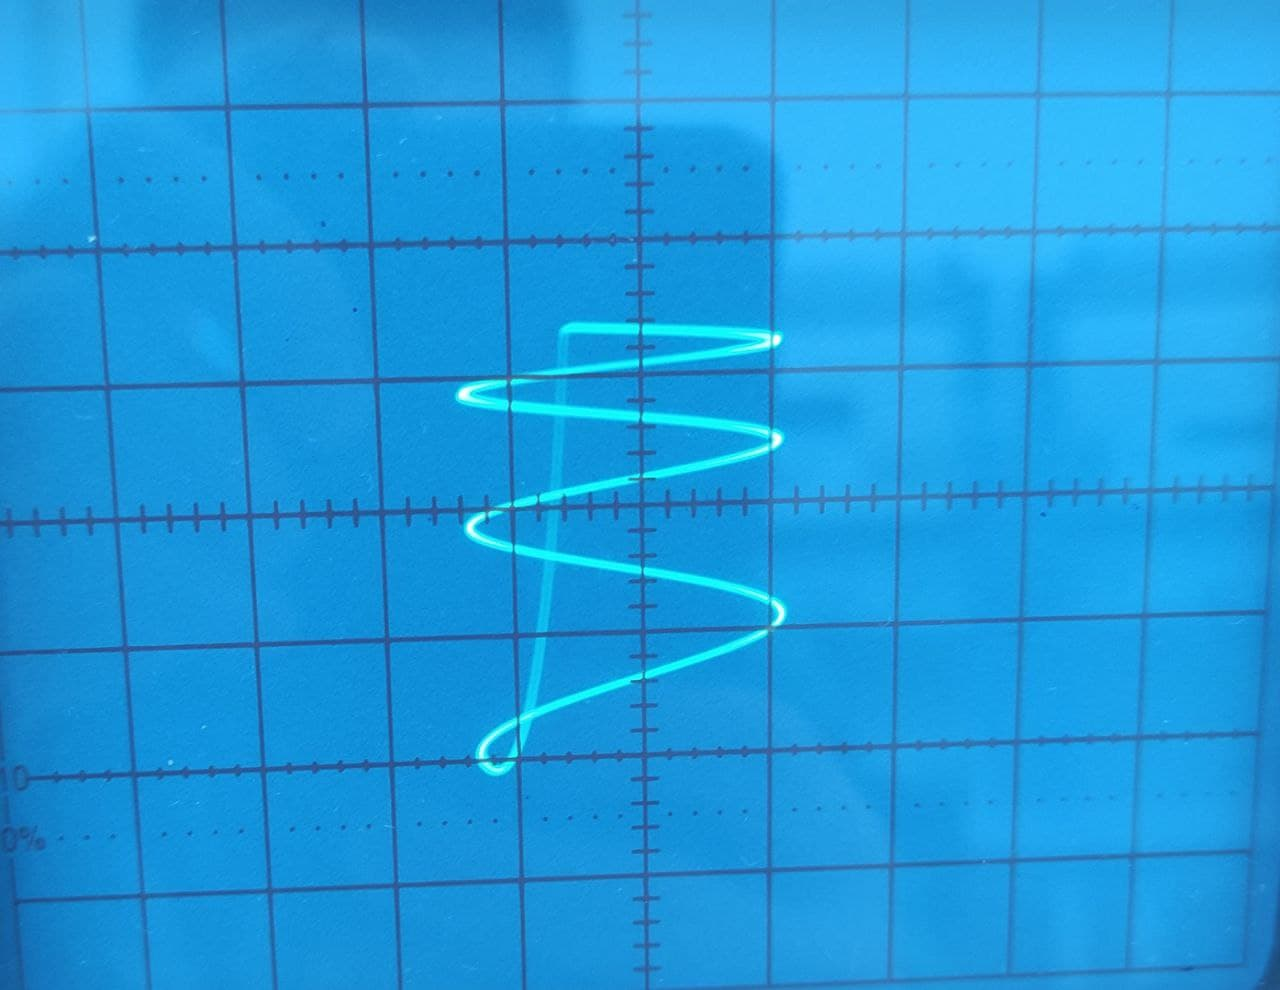
\includegraphics[width=\textwidth]{image_1-3} Соотношение сторон 1:3}
\end{minipage}
\hfill
\begin{minipage}[h]{0.45\linewidth}
	\center{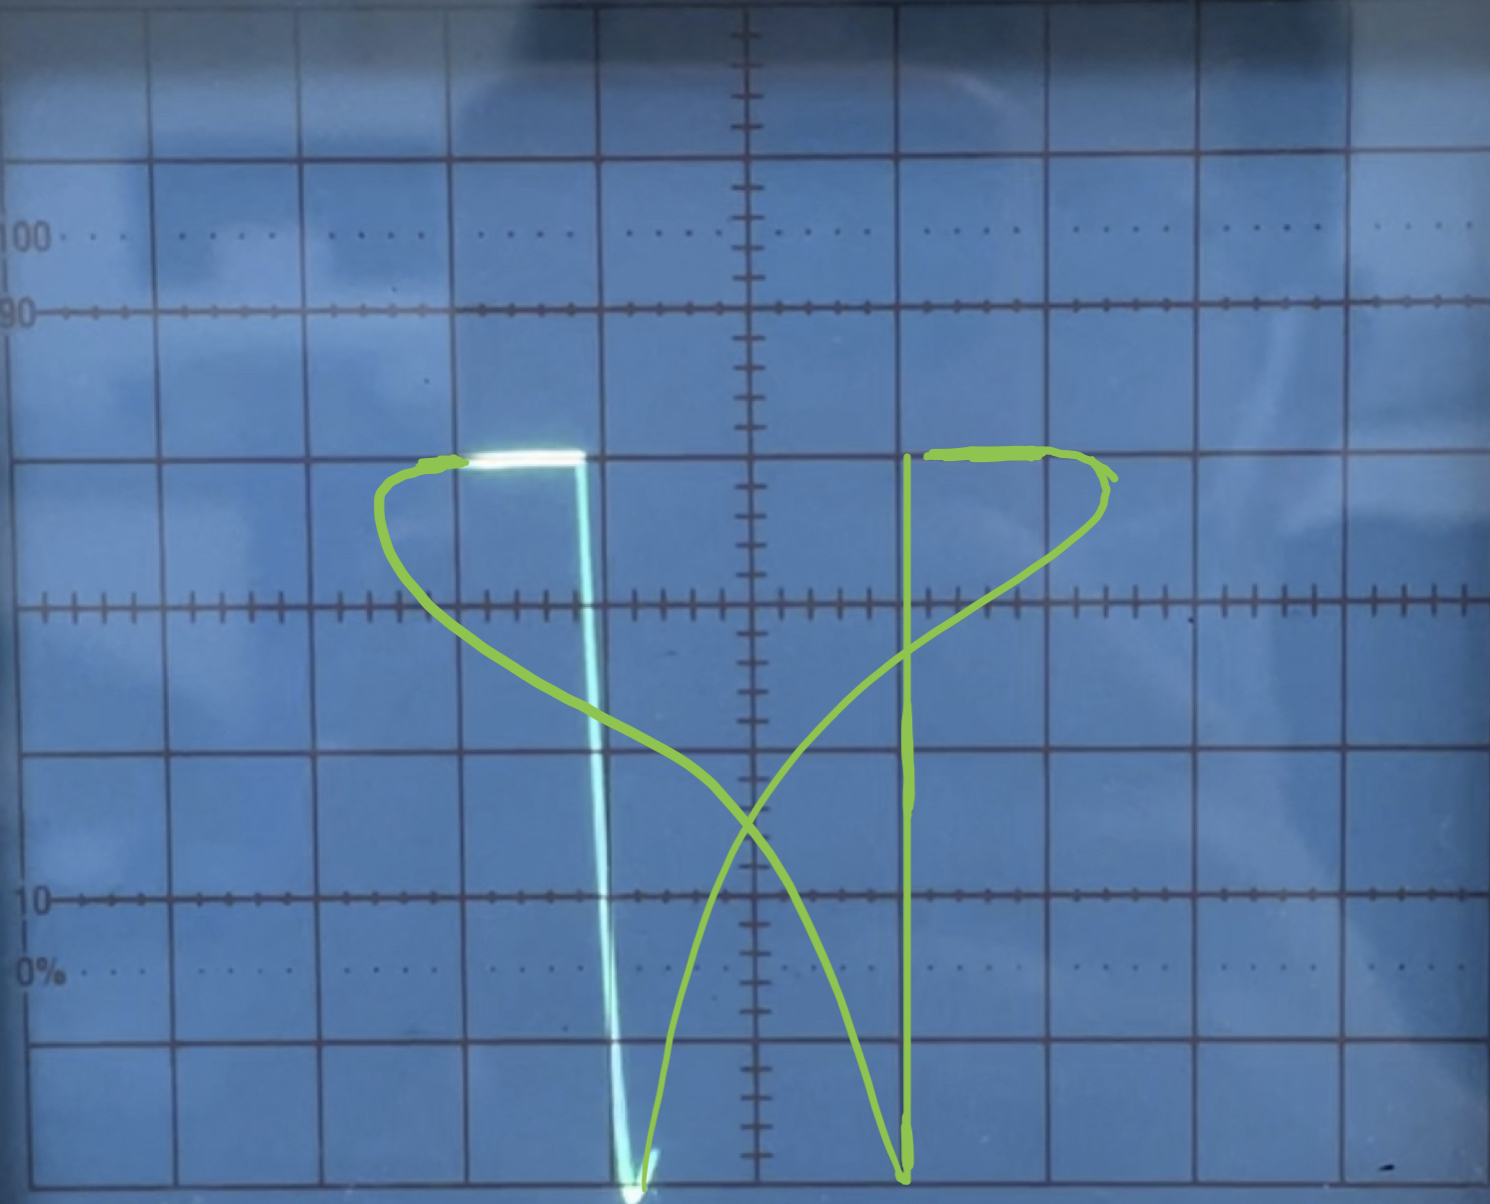
\includegraphics[width=\textwidth]{image_2-1} Соотношение сторон 2:1}
\end{minipage}
\end{figure}

При значении сопротивления $R = 3R_{кр}$ снимем с помощью фигур Лиссажу зависимость частоты колебаний от ёмкости $C$. \\

\begin{figure}[H]
	\begin{minipage}[b]{0.45\linewidth}
		\centering
			\begin{tabular}{|c|c|c|}
				\hline
				\multirow{2}{*}{$C \cdot 10^{-3}$ мкФ} & Теория  & Эксперимент \\ \cline{2-3} 
				& Т, с    & Т, с        \\ \hline
				48                               & 0,00325 & 0,02288     \\ \hline
				42                               & 0,00284 & 0,02004     \\ \hline
				38                               & 0,00257 & 0,01767     \\ \hline
				35                               & 0,00237 & 0,01706     \\ \hline
				40                               & 0,00270 & 0,01873     \\ \hline
				45                               & 0,00304 & 0,02119     \\ \hline
				50                               & 0,00338 & 0,02375     \\ \hline
			\end{tabular}
	\end{minipage}
	\begin{minipage}[b]{0.45\linewidth}
				\centering
		\begin{tabular}{|c|c|c|}
			\hline
			\multirow{2}{*}{R,   кОм} & Теория  & Эксперимент \\ \cline{2-3} 
			& Т, с    & Т, с        \\ \hline
			999999                    & 9,79999 & 0,07143     \\ \hline
			800                       & 0,00784 & 0,05556     \\ \hline
			700                       & 0,00686 & 0,04926     \\ \hline
			600                       & 0,00588 & 0,04167     \\ \hline
			500                       & 0,00490 & 0,03448     \\ \hline
			400                       & 0,00392 & 0,02703     \\ \hline
			300                       & 0,00294 & 0,02028     \\ \hline
			200                       & 0,00196 & 0,01346     \\ \hline
		\end{tabular}
	\end{minipage}	
\end{figure}

Аналогично проведём серию измерений $\nu = f(R)$ при постоянной ёмкости C = 5 $\cdot 10^{-2}$  мкФ,  меняя величину R от максимального значения до критического.
\newpage
По полученным данным построим графики T(R) и T(C):
\begin{figure}[h!]
	\centering
	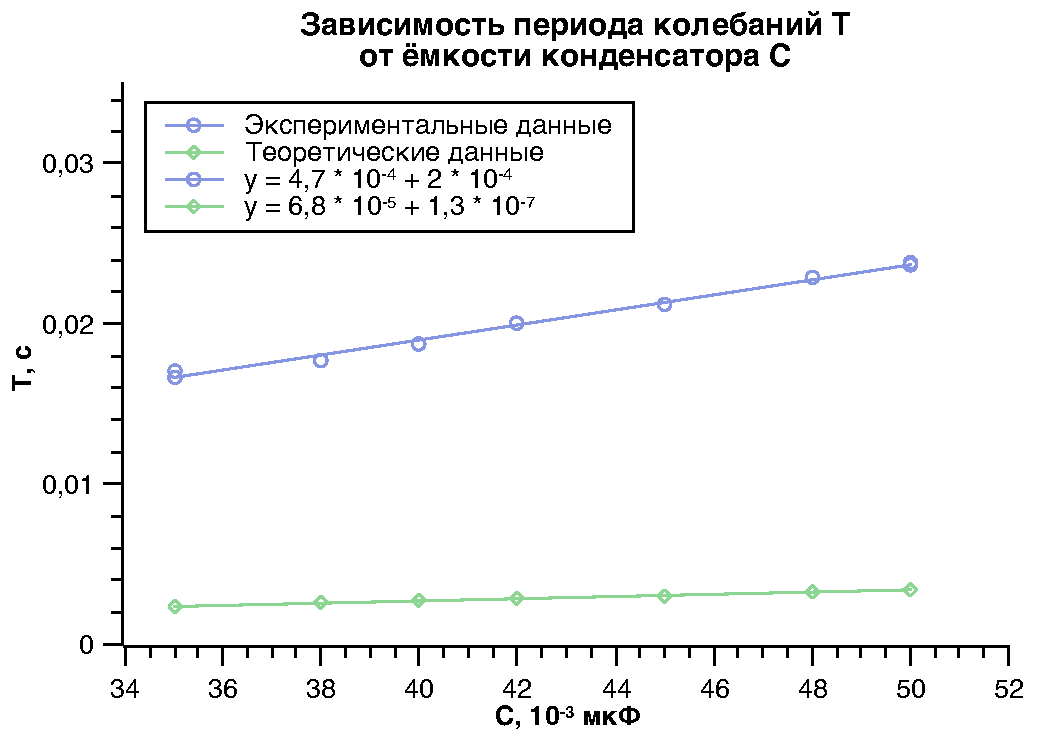
\includegraphics[scale=0.7]{plot_2}
	\caption{Зависимость периода колебаний от ёмкости T(C)}
	\label{fig:plot_2}
\end{figure}
\begin{figure}[h!]
	\centering
	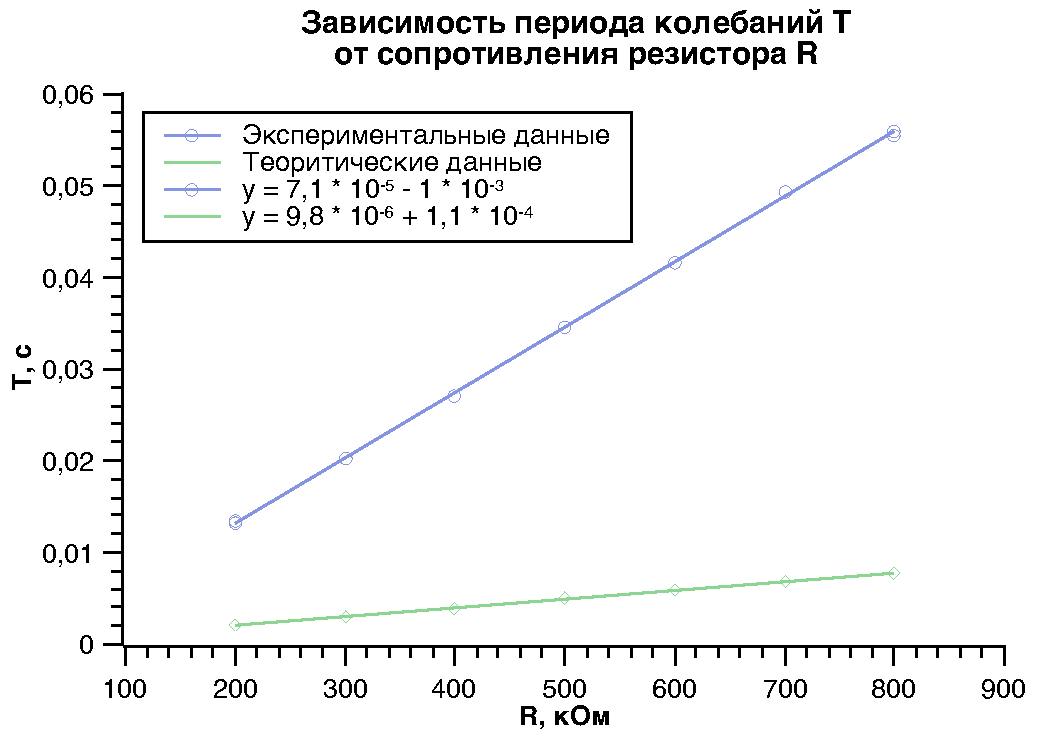
\includegraphics[scale=0.7]{plot_3}
	\caption{Зависимость периода колебаний от ёмкости T(R)}
	\label{fig:plot_3}
\end{figure}


Рассчитаем динамический потенциал гашения для получившихся экспериментальных прямых по формуле: \\
\[
T \approx RC \ln \frac{U - V_2}{U - V_1}
\]
В случае зависимости T(C) получаем $V_2 = 85,7 \, B$, а в случае зависимости T(R) получим $V_2 = 86,2 \, B$

\end{document}